\documentclass{amsart}[12pt]
% \documentclass[times, doublespace]{anzsauth}

\addtolength{\oddsidemargin}{-.75in}%
\addtolength{\evensidemargin}{-.75in}%
\addtolength{\textwidth}{1.5in}%
\addtolength{\textheight}{1.3in}%
\addtolength{\topmargin}{-.8in}%
\addtolength{\marginparpush}{-.75in}%
% \setlength\parindent{0pt}
% \setlength{\bibsep}{0pt plus 0.3ex}

% \usepackage[authoryear]{natbib}
\usepackage{graphicx}
\usepackage{algorithm,algorithmic}
\usepackage{cancel}
\usepackage{amsthm}
\usepackage{mathtools}
\usepackage{algorithm,algorithmic}
\usepackage[inner=2.5cm,outer=1.5cm,bottom=2cm]{geometry}
\usepackage{setspace}
\onehalfspacing
\usepackage{microtype}
\usepackage{color}

\newtheorem{theorem}{Theorem}[section]

\title{Chapter 3 Variational Bayes for Linear Model Selection using Mixtures of g-priors}
\author{Mark Greenaway, John T. Ormerod}

% include.tex
\newcommand{\Bernoulli}[1]{\text{Bernoulli} \left( #1 \right)}
\newcommand{\mydigamma}[1]{\psi \left( #1 \right)}
%\newcommand{\diag}[1]{\text{diag}\left( #1 \right)}
\newcommand{\tr}[1]{\text{tr}\left( #1 \right)}
\newcommand{\Poisson}[1]{\text{Poisson} \left( #1 \right)}
\def \half {\frac{1}{2}}
\def \R {\mathbb{R}}
\def \vbeta {\vec{\beta}}
\def \vy {\vec{y}}
\def \vmu {\vec{\mu}}
\def \vmuqbeta {\vmu_{q(\vbeta)}}
\def \vmubeta {\vmu_{\vbeta}}
\def \Sigmaqbeta {\Sigma_{q(\vbeta)}}
\def \Sigmabeta {\Sigma_{\vbeta}}
\def \va {\vec{a}}
\def \vtheta {\vec{\theta}}
\def \mX {\vec{X}}

\def\ds{{\displaystyle}}

\def\diag{{\mbox{diag}}}


\usepackage{latexsym,amssymb,amsmath,amsfonts}
%\usepackage{tabularx}
\usepackage{theorem}
\usepackage{verbatim,array,multicol,palatino}
\usepackage{graphicx}
\usepackage{graphics}
\usepackage{fancyhdr}
\usepackage{algorithm,algorithmic}
\usepackage{url}
%\usepackage[all]{xy}



\def\approxdist{\stackrel{{\tiny \mbox{approx.}}}{\sim}}
\def\smhalf{\textstyle{\frac{1}{2}}}
\def\vxnew{\vx_{\mbox{{\tiny new}}}}
\def\bib{\vskip12pt\par\noindent\hangindent=1 true cm\hangafter=1}
\def\jump{\vskip3mm\noindent}
\def\etal{{\em et al.}}
\def\etahat{{\widehat\eta}}
\def\thick#1{\hbox{\rlap{$#1$}\kern0.25pt\rlap{$#1$}\kern0.25pt$#1$}}
\def\smbbeta{{\thick{\scriptstyle{\beta}}}}
\def\smbtheta{{\thick{\scriptstyle{\theta}}}}
\def\smbu{{\thick{\scriptstyle{\rm u}}}}
\def\smbzero{{\thick{\scriptstyle{0}}}}
\def\boxit#1{\begin{center}\fbox{#1}\end{center}}
\def\lboxit#1{\vbox{\hrule\hbox{\vrule\kern6pt
      \vbox{\kern6pt#1\kern6pt}\kern6pt\vrule}\hrule}}
\def\thickboxit#1{\vbox{{\hrule height 1mm}\hbox{{\vrule width 1mm}\kern6pt
          \vbox{\kern6pt#1\kern6pt}\kern6pt{\vrule width 1mm}}
               {\hrule height 1mm}}}


%\sloppy
%\usepackage{geometry}
%\geometry{verbose,a4paper,tmargin=20mm,bmargin=20mm,lmargin=40mm,rmargin=20mm}


%%%%%%%%%%%%%%%%%%%%%%%%%%%%%%%%%%%%%%%%%%%%%%%%%%%%%%%%%%%%%%%%%%%%%%%%%%%%%%%%
%
% Some convenience definitions
%
% \bf      -> vector
% \sf      -> matrix
% \mathcal -> sets or statistical
% \mathbb  -> fields or statistical
%
%%%%%%%%%%%%%%%%%%%%%%%%%%%%%%%%%%%%%%%%%%%%%%%%%%%%%%%%%%%%%%%%%%%%%%%%%%%%%%%%

% Sets or statistical values
\def\sI{{\mathcal I}}                            % Current Index set
\def\sJ{{\mathcal J}}                            % Select Index set
\def\sL{{\mathcal L}}                            % Likelihood
\def\sl{{\ell}}                                  % Log-likelihood
\def\sN{{\mathcal N}}                            
\def\sS{{\mathcal S}}                            
\def\sP{{\mathcal P}}                            
\def\sQ{{\mathcal Q}}                            
\def\sB{{\mathcal B}}                            
\def\sD{{\mathcal D}}                            
\def\sT{{\mathcal T}}
\def\sE{{\mathcal E}}                            
\def\sF{{\mathcal F}}                            
\def\sC{{\mathcal C}}                            
\def\sO{{\mathcal O}}                            
\def\sH{{\mathcal H}} 
\def\sR{{\mathcal R}}                            
\def\sJ{{\mathcal J}}                            
\def\sCP{{\mathcal CP}}                            
\def\sX{{\mathcal X}}                            
\def\sA{{\mathcal A}} 
\def\sZ{{\mathcal Z}}                            
\def\sM{{\mathcal M}}                            
\def\sK{{\mathcal K}}     
\def\sG{{\mathcal G}}                         
\def\sY{{\mathcal Y}}                         
\def\sU{{\mathcal U}}  


\def\sIG{{\mathcal IG}}                            


\def\cD{{\sf D}}
\def\cH{{\sf H}}
\def\cI{{\sf I}}

% Vectors
\def\vectorfontone{\bf}
\def\vectorfonttwo{\boldsymbol}
\def\va{{\vectorfontone a}}                      %
\def\vb{{\vectorfontone b}}                      %
\def\vc{{\vectorfontone c}}                      %
\def\vd{{\vectorfontone d}}                      %
\def\ve{{\vectorfontone e}}                      %
\def\vf{{\vectorfontone f}}                      %
\def\vg{{\vectorfontone g}}                      %
\def\vh{{\vectorfontone h}}                      %
\def\vi{{\vectorfontone i}}                      %
\def\vj{{\vectorfontone j}}                      %
\def\vk{{\vectorfontone k}}                      %
\def\vl{{\vectorfontone l}}                      %
\def\vm{{\vectorfontone m}}                      % number of basis functions
\def\vn{{\vectorfontone n}}                      % number of training samples
\def\vo{{\vectorfontone o}}                      %
\def\vp{{\vectorfontone p}}                      % number of unpenalized coefficients
\def\vq{{\vectorfontone q}}                      % number of penalized coefficients
\def\vr{{\vectorfontone r}}                      %
\def\vs{{\vectorfontone s}}                      %
\def\vt{{\vectorfontone t}}                      %
\def\vu{{\vectorfontone u}}                      % Penalized coefficients
\def\vv{{\vectorfontone v}}                      %
\def\vw{{\vectorfontone w}}                      %
\def\vx{{\vectorfontone x}}                      % Covariates/Predictors
\def\vy{{\vectorfontone y}}                      % Targets/Labels
\def\vz{{\vectorfontone z}}                      %

\def\vone{{\vectorfontone 1}}
\def\vzero{{\vectorfontone 0}}

\def\valpha{{\vectorfonttwo \alpha}}             %
\def\vbeta{{\vectorfonttwo \beta}}               % Unpenalized coefficients
\def\vgamma{{\vectorfonttwo \gamma}}             %
\def\vdelta{{\vectorfonttwo \delta}}             %
\def\vepsilon{{\vectorfonttwo \epsilon}}         %
\def\vvarepsilon{{\vectorfonttwo \varepsilon}}   % Vector of errors
\def\vzeta{{\vectorfonttwo \zeta}}               %
\def\veta{{\vectorfonttwo \eta}}                 % Vector of natural parameters
\def\vtheta{{\vectorfonttwo \theta}}             % Vector of combined coefficients
\def\vvartheta{{\vectorfonttwo \vartheta}}       %
\def\viota{{\vectorfonttwo \iota}}               %
\def\vkappa{{\vectorfonttwo \kappa}}             %
\def\vlambda{{\vectorfonttwo \lambda}}           % Vector of smoothing parameters
\def\vmu{{\vectorfonttwo \mu}}                   % Vector of means
\def\vnu{{\vectorfonttwo \nu}}                   %
\def\vxi{{\vectorfonttwo \xi}}                   %
\def\vpi{{\vectorfonttwo \pi}}                   %
\def\vvarpi{{\vectorfonttwo \varpi}}             %
\def\vrho{{\vectorfonttwo \rho}}                 %
\def\vvarrho{{\vectorfonttwo \varrho}}           %
\def\vsigma{{\vectorfonttwo \sigma}}             %
\def\vvarsigma{{\vectorfonttwo \varsigma}}       %
\def\vtau{{\vectorfonttwo \tau}}                 %
\def\vupsilon{{\vectorfonttwo \upsilon}}         %
\def\vphi{{\vectorfonttwo \phi}}                 %
\def\vvarphi{{\vectorfonttwo \varphi}}           %
\def\vchi{{\vectorfonttwo \chi}}                 %
\def\vpsi{{\vectorfonttwo \psi}}                 %
\def\vomega{{\vectorfonttwo \omega}}             %


% Matrices
%\def\matrixfontone{\sf}
%\def\matrixfonttwo{\sf}
\def\matrixfontone{\bf}
\def\matrixfonttwo{\boldsymbol}
\def\mA{{\matrixfontone A}}                      %
\def\mB{{\matrixfontone B}}                      %
\def\mC{{\matrixfontone C}}                      % Combined Design Matrix
\def\mD{{\matrixfontone D}}                      % Penalty Matrix for \vu_J
\def\mE{{\matrixfontone E}}                      %
\def\mF{{\matrixfontone F}}                      %
\def\mG{{\matrixfontone G}}                      % Penalty Matrix for \vu
\def\mH{{\matrixfontone H}}                      %
\def\mI{{\matrixfontone I}}                      % Identity Matrix
\def\mJ{{\matrixfontone J}}                      %
\def\mK{{\matrixfontone K}}                      %
\def\mL{{\matrixfontone L}}                      % Lower bound
\def\mM{{\matrixfontone M}}                      %
\def\mN{{\matrixfontone N}}                      %
\def\mO{{\matrixfontone O}}                      %
\def\mP{{\matrixfontone P}}                      %
\def\mQ{{\matrixfontone Q}}                      %
\def\mR{{\matrixfontone R}}                      %
\def\mS{{\matrixfontone S}}                      %
\def\mT{{\matrixfontone T}}                      %
\def\mU{{\matrixfontone U}}                      % Upper bound
\def\mV{{\matrixfontone V}}                      %
\def\mW{{\matrixfontone W}}                      % Variance Matrix i.e. diag(b'')
\def\mX{{\matrixfontone X}}                      % Unpenalized Design Matrix/Nullspace Matrix
\def\mY{{\matrixfontone Y}}                      %
\def\mZ{{\matrixfontone Z}}                      % Penalized Design Matrix/Kernel Space Matrix

\def\mGamma{{\matrixfonttwo \Gamma}}             %
\def\mDelta{{\matrixfonttwo \Delta}}             %
\def\mTheta{{\matrixfonttwo \Theta}}             %
\def\mLambda{{\matrixfonttwo \Lambda}}           % Penalty Matrix for \vnu
\def\mXi{{\matrixfonttwo \Xi}}                   %
\def\mPi{{\matrixfonttwo \Pi}}                   %
\def\mSigma{{\matrixfonttwo \Sigma}}             %
\def\mUpsilon{{\matrixfonttwo \Upsilon}}         %
\def\mPhi{{\matrixfonttwo \Phi}}                 %
\def\mOmega{{\matrixfonttwo \Omega}}             %
\def\mPsi{{\matrixfonttwo \Psi}}                 %

\def\mone{{\matrixfontone 1}}
\def\mzero{{\matrixfontone 0}}

% Fields or Statistical
\def\bE{{\mathbb E}}                             % Expectation
\def\bP{{\mathbb P}}                             % Probability
\def\bR{{\mathbb R}}                             % Reals
\def\bI{{\mathbb I}}                             % Reals
\def\bV{{\mathbb V}}                             % Reals

\def\vX{{\vectorfontone X}}                      % Targets/Labels
\def\vY{{\vectorfontone Y}}                      % Targets/Labels
\def\vZ{{\vectorfontone Z}}                      %

% Other
\def\etal{{\em et al.}}
\def\ds{\displaystyle}
\def\d{\partial}
\def\diag{\text{diag}}
%\def\span{\text{span}}
\def\blockdiag{\text{blockdiag}}
\def\tr{\text{tr}}
\def\RSS{\text{RSS}}
\def\df{\text{df}}
\def\GCV{\text{GCV}}
\def\AIC{\text{AIC}}
\def\MLC{\text{MLC}}
\def\mAIC{\text{mAIC}}
\def\cAIC{\text{cAIC}}
\def\rank{\text{rank}}
\def\MASE{\text{MASE}}
\def\SMSE{\text{SASE}}
\def\sign{\text{sign}}
\def\card{\text{card}}
\def\notexp{\text{notexp}}
\def\ASE{\text{ASE}}
\def\ML{\text{ML}}
\def\nullity{\text{nullity}}

\def\logexpit{\text{logexpit}}
\def\logit{\mbox{logit}}
\def\dg{\mbox{dg}}

\def\Bern{\mbox{Bernoulli}}
\def\sBernoulli{\mbox{Bernoulli}}
\def\sGamma{\mbox{Gamma}}
\def\sInvN{\mbox{Inv}\sN}
\def\sNegBin{\sN\sB}

\def\dGamma{\mbox{Gamma}}
\def\dInvGam{\mbox{Inv}\Gamma}

\def\Cov{\mbox{Cov}}
\def\Mgf{\mbox{Mgf}}

\def\mis{{mis}} 
\def\obs{{obs}}

\def\argmax{\operatornamewithlimits{\text{argmax}}}
\def\argmin{\operatornamewithlimits{\text{argmin}}}
\def\argsup{\operatornamewithlimits{\text{argsup}}}
\def\arginf{\operatornamewithlimits{\text{arginf}}}


\def\minimize{\operatornamewithlimits{\text{minimize}}}
\def\maximize{\operatornamewithlimits{\text{maximize}}}
\def\suchthat{\text{such that}}


\def\relstack#1#2{\mathop{#1}\limits_{#2}}
\def\sfrac#1#2{{\textstyle{\frac{#1}{#2}}}}


\def\comment#1{
\vspace{0.5cm}
\noindent \begin{tabular}{|p{14cm}|}  
\hline #1 \\ 
\hline 
\end{tabular}
\vspace{0.5cm}
}


\def\mytext#1{\begin{tabular}{p{13cm}}#1\end{tabular}}
\def\mytextB#1{\begin{tabular}{p{7.5cm}}#1\end{tabular}}
\def\mytextC#1{\begin{tabular}{p{12cm}}#1\end{tabular}}

\def\jump{\vskip3mm\noindent}

\def\KL{\text{KL}}
\def\N{\text{N}}
\def\Var{\text{Var}}

\def \E {\mathbb{E}}
\def \BigO {\text{O}}
\def \IG {\text{IG}}
\def \Beta {\text{Beta}}



\newcommand{\mgc}[1]{{\color{blue}#1}}
\newcommand{\joc}[1]{{\color{red}#1}}

\begin{document}

\maketitle

\section*{Abstract}

% What is done in general

We develop mean field and structured variational Bayes approximations for Bayesian model selection on linear
models using Zellner's g prior. Our mean field updates only depend on a single variational parameter $\tau_g$
and other values which are fixed for each model considered. An algorithm is developed which allows these
models to be fit in parallel. Applications to a range of data sets are presented, showing  empirically that
our method performs well on real-world data. Our method is computationally more efficient  than the exact
Bayesian model.

\section{Introduction}

\subsection{Background}

% Problem in general

The problem of model selection is one of the most important problems encountered in practice by applied
statistical practitioners. There are many approaches to model selection including approaches based on
functions of the residual sum of squares, lasso and L1 regression and Bayesian modelling approaches. A major
motivation for this field of research is the need for a computationally feasible approach to performing model
selection on large scale problems where the number of covariates is large.

The bias-variance trade-off is one of the central problems in statistical learning. The guise this problem
takes in model selection is balancing the quality of the model fit against the complexity of the model, in an
attempt to find a compromise between over-fitting and under-fitting, in the hope that the model fit will
generalise well beyond the training data we have observed to the general population and that we haven't simply
learned the noise in the training set.

% Non-Bayesian

Maximising the likelihood alone only maximises the quality of the model fit, without penalising the  model
complexity. There are many approaches to model selection that can be taken. Many model selection criteria have
been proposed to attempt to balance model likelihood and model complexity. One approach to model selection is
to select between entire models, using a model selection criterion. These criterion may have a fixed penalty
for model complexity, such as Akaike's Information Criterion \cite{Akaike1974}, the Risk Inflation Criterion
\cite{Foster1994}, the Schwarz criterion or Bayesian Information Criterion \cite{Schwarz1978}, the Deviance
Information Criterion \cite{Spiegelhalter2016} or the Principle of Minimum Description Length
\cite{Hansen2001}. Alternatively, the penalty may be adaptive/data--dependent \cite{George2000}. An
alternative to model selection criterion is to select models based on their posterior probability, such as by
selecting the median probability model as in \cite{Barbieri2004}.

% Bayesian
Another approach to model selection in a Bayesian context is to use Bayes factors to compare the posterior
likelihoods of the candidate models to see which is most probable given the observed data. This can be done,
for example, by using Bayes Factors as in \cite{Kass1993}.

Yet another approach to model selection is to focus on selecting individual covariates, rather than entire
models. This approach can either be Fully Bayesian or Empirically Bayesian as in \cite{Cui2008}. Variable
selection approaches involve a stochastic search over the variables in the model space. This search can be
driven by posterior probabilities, as in \cite{Casella2006}, or by Gibbs sampling approaches such as in
\cite{George1993}. These two approaches of model selection and variable selection can be combined, as in
\cite{Geweke1996}.

Rather than selecting one candidate model, several models can be combined together using Bayesian model 
averaging, as in \cite{Hoeting1999}, \cite{Raftery1997}, \cite{Fernandez2001} or \cite{Papaspiliopoulos2016}.

Finally, model selection can be made implicit in the model fitting process itself, as in ridge regression
\cite{Casella1980}, of which the well-known lasso is a special case \cite{Tibshirani1996}.

\cite{Zellner1980} suggested a particular form of conjugate Normal-Gamma family where the Bayes factors have a
relatively simple form, incorporating a parameter $g$ to control mixing between the model fit from the data
and a prior specification of model fit. This immediately raises the question of how $g$ should be chosen, and
whether it should be fixed or have a prior specification. \cite{Liang2008} showed that fixed choices of $g$
lead to paradoxes such as Bartlett's Paradox and the Information Paradox, and so a prior specification should
be preferred. There are many ways of choosing a prior on $g$. Using a mixture of $g$-priors has the advantage
of adapting the degree of shrinkage to the prior model dependent on the data.

% Variational Bayes, Explaining Variational Approximations 2010

% VB in general

A challenge to applying this method of model selection is that exact model fitting may be computationally
infeasible for models involving even moderate numbers of observations and covariates, and popular alternatives
for fitting Bayesian models such as Monte Carlo Markov Chains (henceforth referred to as MCMC) are still
extremely computationally intensive. Variational Bayes (see \cite{Ormerod2010}) is a computationally
efficient, deterministic method of fitting Bayesian models to data. Variational Bayes approximates the true
posterior $p(\vy, \vtheta)$ by minimising the KL divergence between the posterior and the  approximating
distribution $q(\vtheta)$.

A linear model with normal priors allows exact inference on the regression and model selection parameters in
closed form, which might appear to negate the beenfits of a variational approximation to the model. However,
the performance of our variational approximation should remain simil.iar if the priors are altered to cater
for complications such as robustness, while exact Bayesian inference calculations are no longer possible
in closed form in these situations.


% Structured Variational Bayes for model selection, Wand and Ormerod Variational Bayes for Elaborate 
% Distributions (\cite{Wand2011})


% Application

% VB theory

% Our main contribution
In this paper, we develop Variational Bayes approximations to model selection of linear models using Zellner's
g prior as in \cite{Liang2008}. We show that in this situation, our variational approximation is almost exact
-- that is, the variational approximation of the Bayesian linear model gives almost perfect estimates.

% By searching of the model space as one covariate changes between each sub-model and  using rank-1 updates on
% $(\mX^\top \mX)^{-1}$, we are able to exhaustively search the model space in $\BigO(2^p np^2)$ rather than
% $\BigO(2^p np^3)$.

This article is organised as follows. In Section \ref{sec:model_selection}, we review previous Bayesian
approaches to model selection. In Section \ref{sec:methodology} we develop our approach. In Section
\ref{sec:num_exp} we perform a series of numerical experiments to show the accuracy of our approach. Finally,
in Section \ref{sec:conclusion}, we provide a Conclusion and Discussion.

\section{Bayesian linear model selection}
\label{sec:model_selection}

Model selection attempts to balance goodness of fit against model complexity, neither overfitting nor
underfitting. Several model selection criteria have been proposed to balance these competing concerns, such as
AIC (\cite{DeLeeuw1992}), BIC (\cite{Schwarz1978}), Mallow's $C_p$ and DIC. As \cite{Breiman1996} and
\cite{Efron2013} showed, while  the standard formulation of a linear model is unbiased, the goodness of fit of
these models is numerically  unstable. Breiman showed that by introducing a penalty on the size of the
regression co- efficients such as  in ridge regression, this numerical instability can be avoided. This reduces
the variances of the co-efficient estimates, at the expense of introducing some bias --- the bias--variance
trade--off.

Consider a normal linear model on $\vy$ with conjugate normal prior on $\vbeta$ with mean centred at $\vzero$,
and covariance $g \sigma^2 (\mX^\top \mX)^{-1}$ where the prior on $g$ is Zellner's g-prior on the covariance
matrices (Zellner 1986), as this yields a tractable posterior for $\vbeta$ as shown by \cite{Liang2008}. We
choose $a$  and $b$ to be $-3/4$ and $(n - p)/2 - a$ respectively, following \cite{Maruyama2011}.

\section{Methodology}
\label{sec:methodology}

\subsection{Notation}

% Definitions

Let $n > 0$ be the number of observations and $p > 0$ be the number of covariates. Let $\vy \in \R^n$ be the
vector of responses, $\vtheta \in \R^p$ be the vector of parameters and $\mX \in \R^{n \times p}$ be the
matrix of covariates. Let $p(\vtheta)$ be the prior distribution of $\vtheta$, $p(\vy, \vtheta)$ be the full
probability distribution of $\vy$, $p(\vtheta | \vy)$ the posterior distribution and $q(\vtheta)$ be the
approximating probability distribution. Let $\kappa$ be the inflation factor such that for the examples under
consideration $n = \kappa p$.

\subsection{Model}

Zellner constructed a family of priors for a Gaussian regression model using a particular form of conjugate
Normal-Gamma model, where the prior covariance matrix of $\vbeta$ is taken to be a multiple of the Fisher
information  matrix by the parameter $g$ \cite{Goel1986}. This places the most prior mass for $\vbeta$ on the
section of the parameter space where the data is least informative.

% \mgc{expand on this? See STAT260 combined lecture notes, page 55}

This leads to the posterior distribution
\[
	\vbeta | \vy \sim \N\left(\frac{g}{1+g} \vbetahatls, g \sigma^2 (\mX^\top \mX)^{-1} \right).
\]

We index the space of models by a $p$-dimensional vector of indicator variables for each variable considered 
for inclusion, $\vgamma$. For each model $\mathcal{M}_\vgamma$, the response vector $\vy$ is modelled by
\begin{equation*}
	\mathcal{M}_\vgamma: \vmu_\vgamma = \vone_n \alpha + \mX_\vgamma \vbeta_\vgamma.
\end{equation*}

Let $\KL(q||p) = \int q(\vtheta) \log{\left( \frac{q(\vtheta)}{p(\vtheta|\vy)} \right)} d \vtheta$ be the
Kuhlback-Leibner divergence between $q$ and $p$, a measure of the distance between the probability
distributions $p$ and $q$.

\subsection{Variational Bayes}

The desired posterior distribution $p(\vtheta | \vy)$ typically requires the calculation of an analytically
intractable integral for all but the simplest models with conjugate priors. Variational Bayes approximates the
full posterior with a simplified approximating distribution $q(\vtheta)$. We relate the true and
approximating distributions as follows:

\begin{align*}
	\log p(\vy) & = \log p(\vy) \int q(\vtheta) d \vtheta = \int q(\vtheta) \log p(\vy) d \vtheta                                    \\
	            & = \int q(\vtheta) \log \left\{ \frac{p(\vy, \vtheta) / q(\vtheta)}{p(\vy|\vtheta) / q(\vtheta)} \right\} d \vtheta \\
	            & = \int q(\vtheta) \log\left\{ \frac{p(\vy, \vtheta)}{q(\vtheta)} \right\} d \vtheta +                              
	\int q(\vtheta) \log\left\{ \frac{q(\vtheta)}{p(\vtheta|\vy)} \right\} d \vtheta \\
	            & = \int q(\vtheta) \log\left\{ \frac{p(\vy, \vtheta)}{q(\vtheta)} \right\} d \vtheta +                              
	\KL(q||p) \\
	            & \geq \int q(\vtheta) \log\left\{ \frac{p(\vy, \vtheta)}{q(\vtheta)} \right\} d \vtheta.                            
\end{align*}

as $\KL(q||p) \geq 0$ for all probability densities $p$ and $q$. The last quantity is the variational lower
bound $\underline{p}(\vtheta) \equiv \int q(\vtheta) \log\left\{ \frac{p(\vy, \vtheta)}{q(\vtheta)} \right\}
d\vtheta$. By the inequality above, this is guaranteed to bound the true probability distribution from below.

The approximation is fit by iteratively maximising the variational lower bound using a sequence of mean field
updates, with each update guaranteed to increase the variational lower bound relative to the previous
iteration. This sequence of mean field updates reduces the KL divergence between the true probability
distribution $p(\vy)$ and the $q(\vtheta)$. The process converges when the variational lower bound no longer
increases. By the above derivation, this can be seen to be equivalent to the KL divergence between the posterior distribution and the approximating distribution being minimised.

A popular form of approximation is to restrict $q(\vtheta)$ to a subclass of product densities by partitioning
$\vtheta = (\vtheta_1, \vtheta_2, \ldots, \vtheta_{M-1}, \vtheta_M)$ and assuming independence between the
partitioned parameters:

\begin{equation*}
	q(\vtheta) \equiv q(\vtheta_1) q(\vtheta_2) \ldots q(\vtheta_{n-1}) q(\vtheta_n).
\end{equation*}

This allows the calculation of the optimal approximating densities $q_i^*(\vtheta_i)$ as

\begin{equation*}
	q_i^*(\vtheta_i) \propto \exp \left \{ \E_{-\vtheta_i} \log p(\vy, \vtheta) \right \}, 1 \leq i \leq M,
\end{equation*}

\subsection{Structured Variational Bayes}

Let $\vgamma \in \{0, 1\}^p$ be the vector of indicators of whether each of the $p$ covariates in our
covariate matrix $\mX$ is included in the model $\vgamma$. We perform model selection by using the above
Variational Bayes approximation to each  candidate linear model and averaging over the space of available
models.

\begin{align*}
	\underline{p}(\vy) & = \sum_\vgamma \underline{p}(\vy|\vgamma) p(\vgamma)                     \\
	p(\vgamma|\vy)     & \approx \frac{\underline{p}(\vy|\vgamma) p(\vgamma)}{\underline{p}(\vy)} \\
	p(\vbeta|\vy)      & \approx \sum_\vgamma q(\vbeta|\vgamma) p(\vgamma|\vy)                    \\
\end{align*}

\subsection{Model}
\label{sec:model}

We consider a linear model with a g-prior, as in \cite{Liang2008}. Consider the linear model

\begin{align*}
	\vy | \vbeta, \sigma^2 \sim \N_n(\mX \vbeta, \sigma^2 \mI) 
\end{align*}

with priors

\begin{align*}
	\vbeta | \sigma^2, g & \sim \N_p(\vzero, g \sigma^2 (\mX^T \mX)^{-1}),                     \\
	p(\sigma^2)          & = (\sigma^2)^{-1} \I(\sigma^2 > 0), \text{ and }                    \\
	p(g)                 & = \frac{g^b (1 + g)^{-(a + b + 2)}}{\Beta(a + 1, b + 1)} \I(g > 0). 
\end{align*}

We choose a factored Variational Bayes approximation of the form
\begin{align*}
	q(\vtheta) = q(\vbeta) q(\sigma^2) q(g). 
\end{align*}

Then $q(\vbeta) = \N(\vmu_{q(\vbeta)}, \mSigma_{q(\vbeta)})$, $q(\sigma^2) = \IG(\alpha_{q(\vbeta)}, \beta_{q(\vbeta)})$ and $q(g) = \text{Beta Prime}(\alpha_{q(g)}, \beta_{q(g)})$.

\subsection{Naive mean field update}
\label{sec:naive_mean_field_updates}

We first present an algorithm for optimising the model fit to the data using mean field updates performed
iteratively on all variational parameters. The derivation of the naive mean field updates is presented in
Appendix \ref{sec:appendix}.

\subsubsection{Numerical integration of $\tau_g$}
\label{sec:num_int}

Define $\tau_{\sigma^2} \equiv \E_q \left[ \sigma^{-2} \right]$ and $\tau_g \equiv \E_q \left[ g^{-1}
\right]$. We can calculate $\tau_g$ numerically using the following iterative numerical scheme.

First, we choose an initial guess $\tau_g^{(1)} = \E_q [g^{-1}] = (1 - R^2) [1 + (p / 2 + a + 1)/b]$. Then
define

\begin{align*}
	\tau_g^{(i+1)} \leftarrow \int_0^\infty g^{\left(b - \frac{p}{2} - 1\right)}                                   
	(1 + g)^{- (a + b + 2)}                                                                                        
	\exp \left \{- \frac{1}{2} g^{-1}  (1 + \tau_g^{(i)})^{-1} [\tau_{\sigma^2} (1 + \tau_g^{(i)})^{-1} n R^2 + p] 
	\right \} dg                                                                                                   
\end{align*}

\noindent where $\tau_{\sigma^2} = [1 - (1 + \tau_g^{(i)})^{-1} R^2]^{-1}$. This integral can be calculated
numerically using Laplace's approximation. This process is repeated until convergence.

Let $\nu - 1 = b - \frac{p}{2}$, 
$\beta = \frac{1}{2} (1 + \tau_g)^{-1} (\tau_{\sigma^2} n R^2 + p)$, 
$\mu - 1 = (a + b + 2)$ and $\gamma = 1$. 

\begin{algorithm}
	\caption{Fit VB approximation of linear model}
	\label{alg:algorithm_one}
	\begin{algorithmic}
		\REQUIRE $\alpha_{q(\sigma^2)} \leftarrow \frac{n + p}{2}, \nu_{q(g)} - 1 \leftarrow b - \frac{p}{2}$, $\mu_{q(g)} - 1 \leftarrow (a + b + 2)$
		\WHILE{the increase in $\log{\underline{p}}(\vy;q)$ is significant}
		\STATE $\vmu_{q(\vbeta)} \leftarrow (1 + \tau_g)^{-1} \vbetahatls$
		\STATE $\mSigma_{q(\vbeta)} \leftarrow [\tau_{\sigma^2} (1 + \tau_g)]^{-1} (\mX^\top \mX)^{-1}$
		\STATE $\beta_{q(\sigma^2)} \leftarrow  \frac{1}{2} {n[1 - (1 + \tau_g)^{-1} R^2] + \tau_{\sigma^2}^{-1} p}$
		\STATE $\beta_{q(g)} \leftarrow \frac{1}{2} (1 + \tau_g)^{-1} [\tau_{\sigma^2} (1 + \tau_g)^{-1} n R^2 + p]$
		\ENDWHILE
	\end{algorithmic}
\end{algorithm}

\subsection{Mean field updates}
\label{sec:mean_field_updates}

A substantially simpler algorithm  which involves optimising over only one variational parameter can be
obtained from Algorithm \ref{alg:algorithm_one} by utlising the following identities.

First, we note that when assuming that $\vy^\top \vy / n = 1$,
\[\vy^\top \mX (\mX^\top \mX)^{-1} \mX^\top \vy =\|\vy\|^2 R^2 = n R^2.\]

Second, observe that when $\vmu = (1 + \tau_g)^{-1} \vbetahatls$ and $\mSigma = \tau_{\sigma^2}^{-1} (1 + \tau_g)^{-1} (\mX^\top \mX)^{-1}$,
\begin{align*}
	\vmu^\top \mX^\top \mX \vmu & = (1 + \tau_g)^{-2} \vbetahatls^\top \mX^\top \mX \vbetahatls                                                        \\
	                            & = (1 + \tau_g)^{-2} \vy^\top \mX (\mX^\top \mX)^{-1} \cancel{\mX^\top \mX} \cancel{(\mX^\top \mX)^{-1}} \mX^\top \vy \\
	                            & = (1 + \tau_g)^{-2} n R^2.                                                                                           
\end{align*}

Third, utilising the above two identities, $s$ can be simplified to
\begin{align*}
	s & = \frac{1}{2} [\|\vy\|^2 - 2 \vmu^\top \mX^\top \vy + (1 + \tau_g) \vmu^\top \mX^\top \mX \vmu (1 + \tau_g) +  \tr (\mX^\top \mX \mSigma)]                 \\
	  & = \frac{1}{2} [n - \cancel{2} (1 + \tau_g) n R ^2 + \cancel{(1 + \tau_g) n R^2} + \tau_{\sigma^2} \tr (\cancel{\mX\top \mX} \cancel{(\mX^\top \mX)^{-1}})] \\
	  & = \frac{1}{2} \{ n[1 - (1 + \tau_g)^{-1} R^2] + p \tau_{\sigma^2}^{-1} \}.                                                                                 
\end{align*}

Fourth, recalling that $\tau_{\sigma^2} = \E_q [\sigma^{-2}] = r/s = \frac{n+p}{n[1 - (1 + \tau_g)^{-1} R^2] + p \tau_{\sigma^2}^{-1}}$, we can solve for $\tau_{\sigma^2}$ in terms of $\tau_g$ to obtain
\[
	\tau_{\sigma^2} = [1 + (1 + \tau_g)^{-1}]^{-1}.
\]

Hence

\begin{align*}
	s & = \frac{r}{\tau_{\sigma^2}} = \frac{1}{2} (n + p) [1 - (1 + \tau_g)^{-1} R^2], \text{ and }                \\
	c & = \frac{\tau_{\sigma^2}}{2}[\vmu^\top \mX^\top \mX \vmu + \tr (\mX^\top \mX \mSigma)]                      \\
	  & = \frac{\tau_{\sigma^2}}{2}\left[(1 + \tau_g)^{-2} n R^2 + \tau_{\sigma^2}^{-1} (1 + \tau_g)^{-1} p\right] \\
	  & = \frac{1}{2} [ \tau_{\sigma^2} (1 + \tau_g)^{-2} n R^2 + (1 + \tau_g)^{-1} p]                             \\
	  & = \frac{1}{2} \{ [1 + (1 + \tau_g)^{-1}]^{-1} (1 + \tau_g)^{-2} n R^2 + (1 + \tau_g)^{-1} p\}.             
\end{align*}

\noindent Hence all of the variational parameter updates in Algorithm \ref{alg:algorithm_one} can be expressed as functions
of $n$, $p$, $R^2$ and $\tau_g$. Thus optimisation can be performed on $\tau_g$ alone by repeatedly using the
scheme presented in \ref{sec:num_int}. Once $\tau_g$ is fully optimised, the other variational parameters can
be calculated from it as shown in Algorithm \ref{alg:algorithm_two}.

\begin{algorithm}
	\caption{Fit VB approximation of linear model}
	\label{alg:algorithm_two}
	\begin{algorithmic}
		\REQUIRE $\nu_{q(g)} - 1 \leftarrow b - \frac{p}{2}$, $\mu_{q(g)} - 1 \leftarrow (a + b + 2)$ \\
		\WHILE{the increase in $\log{\underline{p}}(\vy;q)$ is significant}
		\STATE Calculate $\tau_{g}$ using numerical integration in Section \ref{sec:num_int}
		\ENDWHILE
		\STATE $\tau_{\sigma^2} \leftarrow \{[1 - (1 + \tau_g)^{-1}] R^2\}^{-1}$
		\STATE $\beta_{q(g)} \leftarrow \left(\frac{n (1 + \tau_g)^{-1}}{[1 - (1 + \tau_g)^{-1}]} + p \right)$
		\STATE $\vmu_{q(\vbeta)} \leftarrow (1 + \tau_g)^{-1} (\mX^\top \mX)^{-1} \mX^\top \vy$
		\STATE $\mSigma_{q(\vbeta)} \leftarrow \tau_{\sigma^2}^{-1} (1 + \tau_{g})^{-1}(\mX^\top \mX)^{-1}$
	\end{algorithmic}
\end{algorithm}

\section{Numerical experiments}
\label{sec:num_exp}

To assess the accuracy of our variational approximations to the exact posteriors, we examined a number of
measures. All of the measures that we examined were functions of $\kappa$, $p$ and $R^2$, and so serve to
characterise the performance of our approximation on any possible data set with a number of observations
$n$, number of covariates $p$ and correlation $R$ between the response $\vy$ and the covariate matrix $\mX$.

\subsection{Shrinkage}

Exact posterior and approximate shrinkage $\left( \frac{g}{1 + g} \right)$ were calculated for a range of
values of $p$, $n$ and $R^2$ to compare their values. As can be seen from Figure $\ref{fig:shrinkage}$, the
values of the exact posterior shrinkage and approximate shrinkage are almost the same over most of the range
of these values, with deviation only noticeable in the $p=10$ and $p=20$ cases.

\begin{figure}[p]
	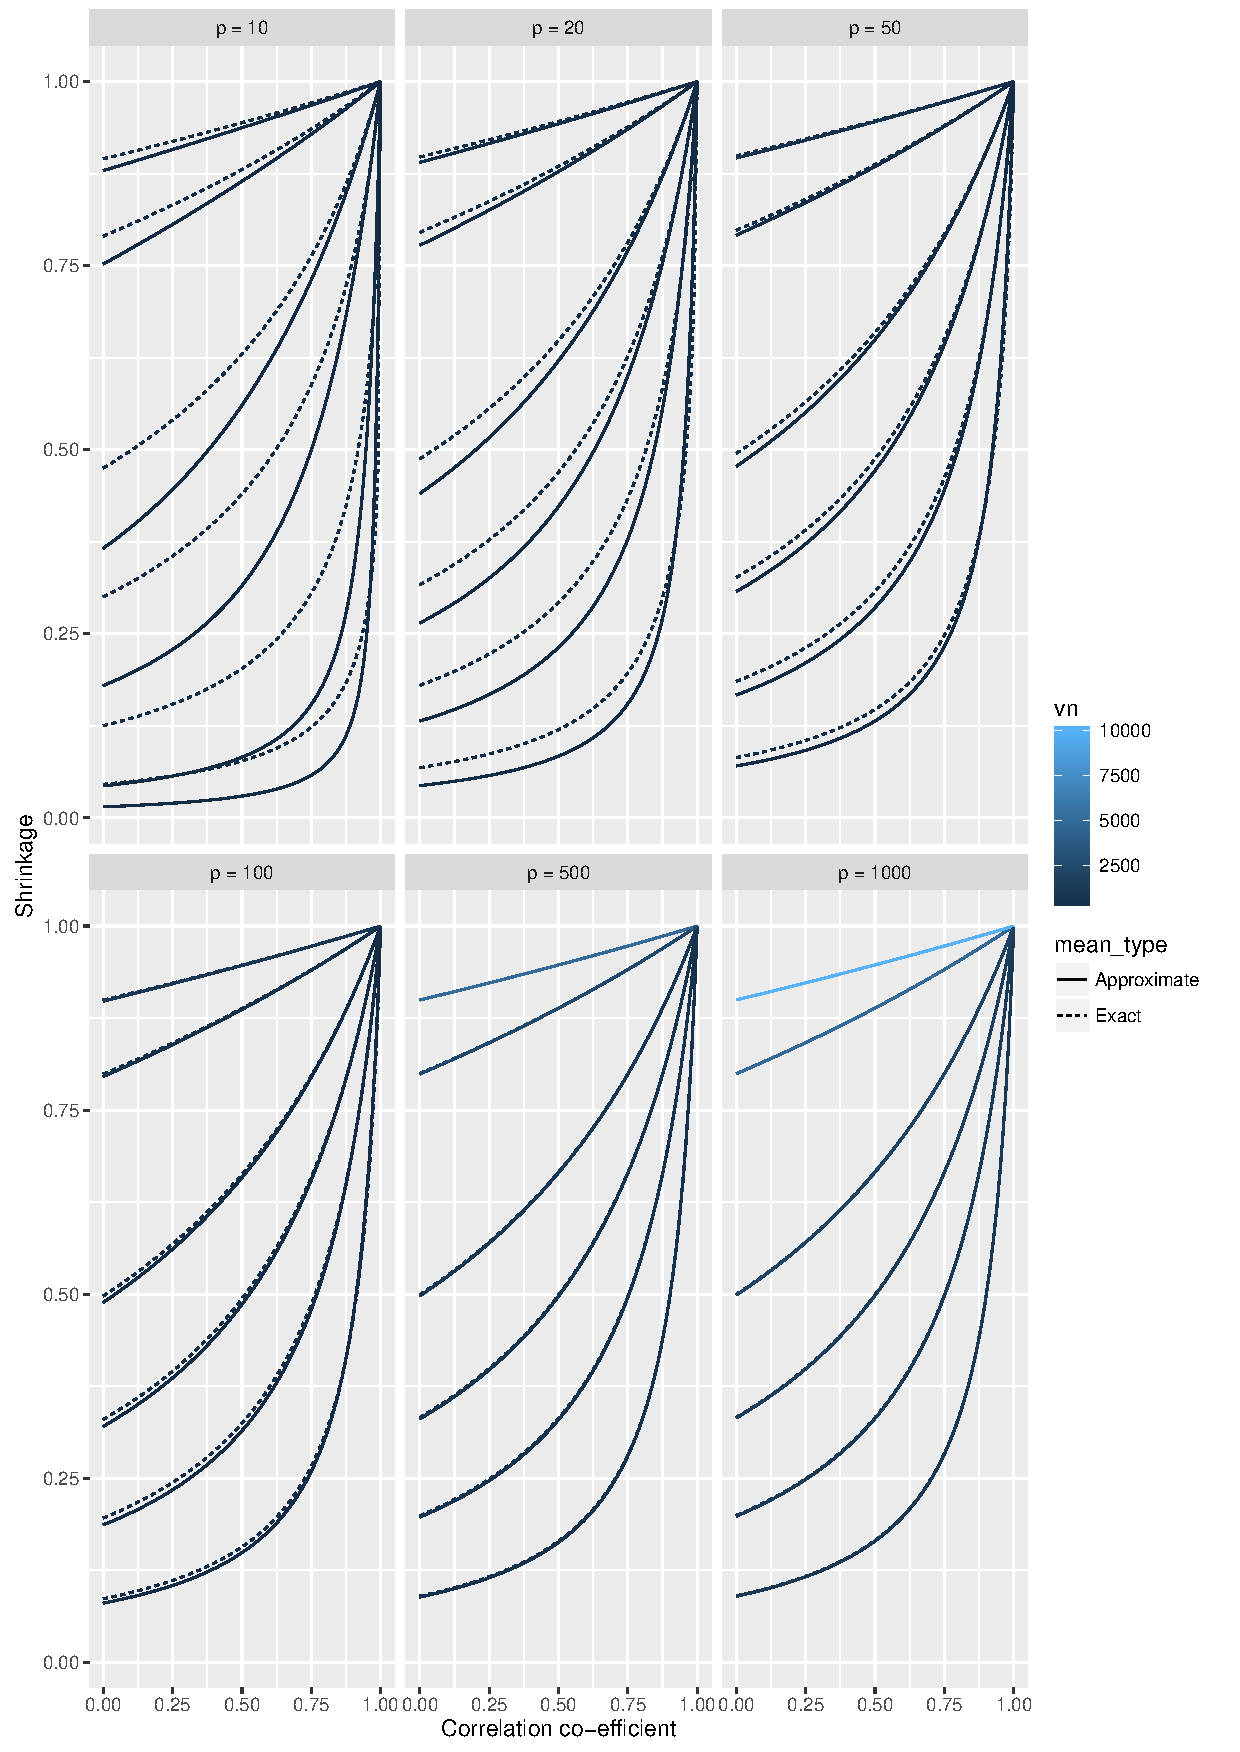
\includegraphics[width=17cm, height=17cm]{Chapter_3_shrinkage.pdf}
	\caption{The ratio $\frac{g}{1 + g} | \vy$ controls the degree to which the model fit tends back towards
		the prior mean. This ratio is approximated in the variational approximation by $(1 + \tau_g^{-1})^{-1}$. We
	compare these two quantities in the figure above.}
	\label{fig:shrinkage}
\end{figure}

Coefficient posterior variance \\

We can see from Figure \ref{fig:variance} that as $p$ and $\kappa$ increase, the approximation to the
posterior variance of \ldots becomes more and more accurate.

\begin{figure}[p]
	\includegraphics[width=17cm, height=17cm]{code/taug/Variance.pdf}
	\caption{The posterior variance of the example model $p(\sigma^2 | \vy)$ is compared against the approximation
		to the posterior variance $q(\sigma^2)$ across a range of numbers of covariates, sample sizes and $R^2$
	values.}
	\label{fig:variance}
\end{figure}

Accuracy of approximation to $p(\sigma^2 | \vy)$ \\

We assessed the accuracy of the approximation to $p(\sigma^2 | \vy)$ by $q(\sigma^2)$ by numerically evaluating
the integral
\[
	1 - \frac{1}{2} \int_0^\infty |p(\sigma^2 | \vy) - q(\sigma^2)| d \sigma^2
\]
for a range of values of $p$, $\kappa$ and $R^2$. The results are presented in Figure \ref{fig:accuracy_sigma2}.

\begin{figure}[p]
	\includegraphics[width=17cm, height=17cm]{code/taug/Accuracy_sigma2.pdf}
	\caption{The accuracy of the approximation $q(\sigma^2)$ is assessed by computing the integral   $1 -
		\frac{1}{2} \int_0^\infty |p(\sigma^2 | \vy) - q(\sigma^2)| d \sigma^2$ and graphing the result over a range
	of numbers of covariates, sample sizes and $R^2$  values.}
	\label{fig:accuracy_sigma2}
\end{figure}

Accuracy of approximation to $p(g | \vy)$ \\

\begin{figure}[p]
	\includegraphics[width=17cm, height=17cm]{code/taug/Accuracy_g.pdf}
	\caption{The accuracy of the approximation $q(g)$ is assessed by computing the integral   $1 -
		\frac{1}{2} \int_0^\infty |p(g | \vy) - q(g)| d g$ and graphing the result over a range
	of numbers of covariates, sample sizes and $R^2$  values.}
	\label{fig:accuracy_g}
\end{figure}

We assessed the accuracy of the approximation to $p(g | \vy)$ by $q(g)$ by numerically evaluating the integral
\[
	1 - \frac{1}{2} \int_0^\infty |p(g | \vy) - q(g)| d g
\]
for a range of values of $p$, $\kappa$ and $R^2$. The results are presented in Figure \ref{fig:accuracy_g}.


$\log{p(\vy)}$ versus ELBO \\

We assessed the accuracy of the variational lower bound by calculating the relative error of
$\log{\underline{p}(\vy)}$ versus $\log{p(\vy)}$. The results are presented in Figure
\ref{fig:relative_error}.

\begin{figure}[p]
	\includegraphics[width=17cm, height=17cm]{code/taug/Relative_error_log_p.pdf}
	\caption{Relative error of the variational lower bound versus $\log{p(\vy)}$}
	\label{fig:relative_error}
\end{figure}

Precision \\

The accuracy of the precision was assessed by calculating the relative error of the approximate precision
versus the exact posterior precision. The results are presented in Figure \ref{fig:precision}. As $p$ and
$\kappa$ increase, we can see that the approximate precision is converging towards the exact precision for all
values of $R^2$.

\begin{figure}[p]
	\includegraphics[width=17cm, height=17cm]{code/taug/Precision.pdf}
	\caption{Relative error of the approximate posterior precision versus the exact posterior precision}
	\label{fig:precision}
\end{figure}

\subsection{Marginal covariate inclusion probabilities}

The marginal covariate inclusion probabilities from the variational approximation match those from the the
exact posterior likelihood very closely. Comparing these marginal covariate inclusion probabilities to those
produced by weighting each model considered by AIC and BIC, we see that the probabilities produced by the
variational approximation and exact posterior likelihood are more conservative.

\begin{figure}[p]
	\includegraphics[width=17cm, height=17cm]{code/taug/Log_of_Relative_error_of_Variance_of_g.pdf}
	\caption{Log of the relative error of the approximate variance of g relative to the exact variance of g}
	\label{fig:rel_error_var_g}
\end{figure}


% vw1 <- read.csv("Hitters_vw1.csv", header=FALSE)
% r <- hist(as.matrix(vw1), breaks=19, axes=FALSE, prob=TRUE, main="", xlab="")
% axis(1, r$mid, c("1", "2", "3", "4", "5", "6", "7", "8", "9", "10", "11", "12", "13", "14", "15", "16", "17", "18"))

% bodyfat
% Major League Baseball Data from the 1986 and 1987 seasons.
% An Introduction to Statistical Learning with Applications in R

% \begin{tabular}{|l|lllllllllllllllllll|}
% 	\hline
% 	$\vp$ & 0.137 & 0.130 & 0.257 & 0.982 & 0.921 & 0.173 & 0.633 & 0.562 & 0.623 & 0.480 & 0.441 & 0.499 & 0.197 & 0.926 & 0.131 & 0.174 & 0.128 & 0.901 & 0.851 \\
% 	$\vq$ & 0.137 & 0.130 & 0.257 & 0.982 & 0.922 & 0.172 & 0.635 & 0.562 & 0.625 & 0.480 & 0.440 & 0.499 & 0.197 & 0.927 & 0.130 & 0.173 & 0.127 & 0.902 & 0.853 \\
% 	\hline
% \end{tabular}

\subsubsection{Hitters}

The Hitters data set was taken from the StatLib library maintained by Carnegie Mellon University, and used in
\cite{James:2014:ISL:2517747}. The data was gathered from the the performance of players during the Major
League Baseball seasons for 1986 and 1987, and includes the following covariates:

\begin{tabular}{|ll|}
	\hline
	Covariate & Description                                                                        \\
	\hline
	AtBat     & Number of times at bat in 1986                                                     \\
	Hits      & Number of hits in 1986                                                             \\
	HmRun     & Number of home runs in 1986                                                        \\
	Runs      & Number of runs in 1986                                                             \\
	RBI       & Number of runs batted in in 1986                                                   \\
	Walks     & Number of walks in 1986                                                            \\
	Years     & Number of years in the major leagues                                               \\
	CAtBat    & Number of times at bat during his career                                           \\
	CHits     & Number of hits during his career                                                   \\
	CHmRun    & Number of home runs during his career                                              \\
	CRuns     & Number of runs during his career                                                   \\
	CRBI      & Number of runs batted in during his career                                         \\
	CWalks    & Number of walks during his career                                                  \\
	League    & A factor with levels A and N indicating player’s league at the end of 1986       \\
	Division  & A factor with levels E and W indicating player’s division at the end of 1986     \\
	PutOuts   & Number of put outs in 1986                                                         \\
	Assists   & Number of assists in 1986                                                          \\
	Errors    & Number of errors in 1986                                                           \\
	Salary    & 1987 annual salary on opening day in thousands of dollars                          \\
	NewLeague & A factor with levels A and N indicating player’s league at the beginning of 1987 \\
	\hline
\end{tabular}

The marginal covariate inclusion probabilities are presented in Figure \ref{fig:Hitters_inclusion}.

\begin{figure}[p]
	\includegraphics[scale=.4]{Hitters_variable_selection.pdf}
	\caption{Hitters marginal inclusion probablities}
	\label{fig:Hitters_inclusion}
\end{figure}

The model ranking scatterplots are presented in Figure \ref{fig:Hitters_model_ranking}.



\begin{figure}[p]
	\includegraphics[scale=.4]{code/Model_selection_scatter_plot_1.pdf}
	\caption{Hitters model ranking scatterplot}
	\label{fig:Hitters_model_ranking}
\end{figure}

\subsubsection{Body Fat}
The Body Fat data set was taken from \cite{Tarr2015}, and is on the relationship between percentage of body
fat and simple body measurements. The data set consists of 128 observations, and the covariates in the data set
are:

\begin{tabular}
	\hline
	Covariate & Description                                                                  \\
	\hline
	Id        & Identifier                                                                   \\
	Bodyfat   & Bodyfat percentage                                                           \\
	Age       & Age (years)                                                                  \\
	Weight    & Weight (kg)                                                                  \\
	Height    & Height (inches)                                                              \\
	Neck      & Neck circumference (cm)                                                      \\
	Chest     & Chest circumference (cm)                                                     \\
	Abdo      & Abdomen circumference (cm) "at the umbilicus and level with the iliac crest" \\
	Hip       & Hip circumference (cm)                                                       \\
	Thigh     & Thigh circumference (cm)                                                     \\
	Knee      & Knee circumference (cm)                                                      \\
	Ankle     & Ankle circumference (cm)                                                     \\
	Bic       & Extended biceps circumference (cm)                                           \\
	Fore      & Forearm circumference (cm)                                                   \\
	Wrist     & Wrist circumference (cm) "distal to the styloid processes"                   \\
	\hline
\end{tabular}

The marginal covariate inclusion probabilities are presented in Figure \ref{fig:bodyfat_inclusion}.

% \begin{tabular}{|l|lllllllllllll|}
% 	\hline
% 	$\vp$ & 0.938 & 0.136 & 0.182 & 0.072 & 0.071 & 0.108 & 0.147 & 1.000 & 0.134 & 0.141 & 0.323 & 0.619 & 0.221 \\
% 	$\vq$ & 0.939 & 0.136 & 0.182 & 0.071 & 0.070 & 0.107 & 0.146 & 1.000 & 0.134 & 0.140 & 0.323 & 0.620 & 0.221 \\
% 	\hline
% \end{tabular}

\begin{figure}[p]
	\includegraphics[scale=.4]{bodyfat_variable_selection.pdf}
	\caption{bodyfat marginal inclusion probablities}
	\label{fig:bodyfat_inclusion}
\end{figure}

The model ranking scatterplots are presented in Figure \ref{fig:bodyfat_model_ranking}.

\begin{figure}[p]
	\includegraphics[scale=.4]{code/Model_selection_scatter_plot_2.pdf}
	\caption{bodyfat model ranking scatterplot}
	\label{fig:bodyfat_model_ranking}
\end{figure}

\subsubsection{Wage}

The Wage gap data set was taken from \cite{James:2014:ISL:2517747}, on 3000 workers in the Mid-Atlantic
region. The data set includes 12 covariates:

\begin{tabular}{|ll|}
	\hline
	Covariate        & Description                                                                           \\
	\hline
	Year             & Year that the wage information was recorded                                           \\
	Age              & Age of worker                                                                         \\
	Sex              & Gender                                                                                \\
	Marital status   & Marital status -- Never Married, Married, Widowed, Divorced or Seperated              \\
	Race             & White, Black, Asian or Other                                                          \\
	Education        & Education level -- Did not graduate high school, Graduated high school, Some College, 
	College Graduate \\
	                 & or Advanced College Degree                                                            \\
	Region           & Region of the country                                                                 \\
	Job class        & Type of job                                                                           \\
	Health           & Either Good or Less, or Very Good or Better                                           \\
	Health insurance & Yes or No                                                                             \\
	Log of wage      & The log of the worker's wage                                                          \\
	Wage             & The worker's wage                                                                     \\
	\hline
\end{tabular}

The marginal covariate inclusion probabilities are presented in Figure \ref{fig:Wage_inclusion}.

% \begin{tabular}{|l|lllllllllllllllll|}
% 	\hline
% 	$\vp$ & 1 & 1 & 0.010 & 0.024 & 1 & 0.054 & 0.083 & 0.019 & 0.011 & 0.010 & 0.013 & 0.014 & 0.011 & 0.014 & 0.057 & 0.042 & 0.033 \\
% 	$\vq$ & 1 & 1 & 0.010 & 0.024 & 1 & 0.054 & 0.083 & 0.019 & 0.011 & 0.010 & 0.013 & 0.014 & 0.011 & 0.014 & 0.057 & 0.042 & 0.033 \\
% 	\hline
% \end{tabular}

\begin{figure}[p]
	\includegraphics[scale=.4]{Wage_variable_selection.pdf}
	\caption{Wage marginal inclusion probablities}
	\label{fig:Wage_inclusion}
\end{figure}

The model ranking scatterplots are presented in Figure \ref{fig:Wage_model_ranking}.

\begin{figure}[p]
	\includegraphics[scale=.4]{code/Model_selection_scatter_plot_3.pdf}
	\caption{Wage model ranking scatterplot}
	\label{fig:Wage_model_ranking}
\end{figure}


\subsubsection{Graduation Rate}

The Graduation Rate data set was taken from \cite{James:2014:ISL:2517747}. The data is drawn from the 1995
issue of US News and World Report, and is on a large number of US Colleges. The data set consists of 777
observations, and includes the following covariates:

\begin{tabular}{|ll|}
	\hline
	Covariate   & Description                                                             \\
	\hline
	Private     & A factor with levels No and Yes indicating private or public university \\
	Apps        & Number of applications received                                         \\
	Accept      & Number of applications accepted                                         \\
	Enroll      & Number of new students enrolled                                         \\
	Top10perc   & Percentage of new students from top 10\% of H.S. class                  \\
	Top25perc   & Percentage of new students from top 25\% of H.S. class                  \\
	F.Undergrad & Number of fulltime undergraduates                                       \\
	P.Undergrad & Number of parttime undergraduates                                       \\
	Outstate    & Out-of-state tuition                                                    \\
	Room.Board  & Room and board costs                                                    \\
	Books       & Estimated book costs                                                    \\
	Personal    & Estimated personal spending                                             \\
	PhD         & Percentage of faculty with Ph.D.’s                                    \\
	Terminal    & Percentage of faculty with terminal degree                              \\
	S.F.Ratio   & Student/faculty ratio                                                   \\
	perc.alumni & Percentage of alumni who donate                                         \\
	Expend      & Instructional expenditure per student                                   \\
	Grad.Rate   & Graduation rate                                                         \\
	\hline
\end{tabular}

The marginal covariate inclusion probabilities are presented in Figure \ref{fig:GradRate_inclusion}.

% \begin{tabular}{|l|lllllllllllllllll|}
% 	\hline
% 	$\vp$ & 0.913 & 1.000 & 0.090 & 0.108 & 0.110 & 0.602 & 0.127 & 0.945 & 0.999 & 0.999 & 0.201 & 0.864 & 0.262 & 0.105 & 0.146 & 0.977 & 0.437 \\
% 	$\vq$ & 0.914 & 1.000 & 0.090 & 0.108 & 0.110 & 0.602 & 0.127 & 0.945 & 0.999 & 0.999 & 0.201 & 0.864 & 0.262 & 0.105 & 0.146 & 0.977 & 0.437 \\
% 	\hline
% \end{tabular}

\begin{figure}[p]
	\includegraphics[scale=.4]{GradRate_variable_selection.pdf}
	\caption{GradRate marginal inclusion probablities}
	\label{fig:GradRate_inclusion}
\end{figure}

The model ranking scatterplots are presented in Figure \ref{fig:GradRate_model_ranking}.

\begin{figure}[p]
	\includegraphics[scale=.4]{code/Model_selection_scatter_plot_4.pdf}
	\caption{GradRate model ranking scatterplot}
	\label{fig:GradRate_model_ranking}
\end{figure}

\subsubsection{US Crime}
The US Crime data set was taken from the \texttt{MASS} package \cite{Venables2002}, and is on the effect of
punishment regimes on crime rates. The data set includes 47 states of the United States of America. The
variables have been re-scaled for convenience, and include the following covariates:

\begin{tabular}{|ll|}
	\hline
	Covariate & Description                                                     \\
	\hline
	M         & percentage of males aged 14–24.                               \\
	So        & indicator variable for a Southern state.                        \\
	Ed        & mean years of schooling.                                        \\
	Po1       & police expenditure in 1960.                                     \\
	Po2       & police expenditure in 1959.                                     \\
	LF        & labour force participation rate.                                \\
	M.F       & number of males per 1000 females.                               \\
	Pop       & state population.                                               \\
	NW        & number of non-whites per 1000 people.                           \\
	U1        & unemployment rate of urban males 14–24.                       \\
	U2        & unemployment rate of urban males 35–39.                       \\
	GDP       & gross domestic product per head.                                \\
	Ineq      & income inequality.                                              \\
	Prob      & probability of imprisonment.                                    \\
	Time      & average time served in state prisons.                           \\
	y         & rate of crimes in a particular category per head of population. \\
	\hline
\end{tabular}

The marginal covariate inclusion probabilities are presented in Figure \ref{fig:USCrime_inclusion}.

% \begin{tabular}{|l|lllllllllllllll|}
% 	\hline
% 	$\vp$ & 0.226 & 0.849 & 0.997 & 0.216 & 0.502 & 0.244 & 0.358 & 0.569 & 0.324 & 0.202 & 0.424 & 0.696 & 0.869 & 0.229 & 0.655 \\
% 	$\vq$ & 0.220 & 0.856 & 0.997 & 0.210 & 0.507 & 0.240 & 0.358 & 0.573 & 0.318 & 0.196 & 0.418 & 0.699 & 0.876 & 0.224 & 0.661 \\
% 	\hline
% \end{tabular}

\begin{figure}[p]
	\includegraphics[scale=.4]{USCrime_variable_selection.pdf}
	\caption{USCrime marginal inclusion probablities}
	\label{fig:USCrime_inclusion}
\end{figure}

The model ranking scatterplots are presented in Figure \ref{fig:USCrime_model_ranking}.

\begin{figure}[p]
	\includegraphics[scale=.4]{code/Model_selection_scatter_plot_5.pdf}
	\caption{USCrime model ranking scatterplot}
	\label{fig:USCrime_model_ranking}
\end{figure}

\section{Conclusion and Discussion}
\label{sec:conclusion}

The Variational Bayes approximation produces results which are almost identical to the exact likelihood.
The VB metholodology extends naturally to new situations, such as robust model fitting, mixed effects, missing
data, measurement error and splines. We are able to retain high accuracy with less computational overhead than
exact or MCMC.

All of the variational parameters in Algorithm \ref{alg:algorithm_two} except $\tau_g$ depend only on
$\tau_g$ and the fixed quantities $n$, $p$, $R^2$, $\mX$ and $\vy$. This allows us to optimise $\tau_g$
only, and then set the rest of the variational parameters at the end of the algorithm. The fact that only
univariate optimisation is required reduces the computation required to fit our approximation considerably,
which makes this algorithm applicable when speed and/or the ability to parallelise the algorithm are
paramount, such as model selection via structured Variational Bayes.

\bibliographystyle{elsarticle-harv}
\bibliography{references_mendeley}

\appendix
\section{Derivation of Naive Mean Field Updates}
\label{sec:appendix}

\end{document}